% ===== §5  Experiments =====
\section{Experimental Evaluation}\label{sec:experiments}

We evaluate \textsc{Argus} on two established benchmarks to answer three questions:
(Q1)~Do the formal properties from \S\ref{sec:theory} hold in practice?
(Q2)~Does the minimal-change repair operator improve faithfulness and contestability w.r.t.\ existing baselines?
(Q3)~What is the empirical cost of repair?

We evaluate on 500 randomly sampled instances (seed 42) from HotpotQA~\cite{yang2018hotpotqa}, a multi-hop question answering dataset, and 500 instances from FEVER~\cite{thorne2018fever}, a fact verification dataset.
For each instance, evidence updates~$\Delta$ are constructed from the gold supporting facts: we withhold one fact during initial explanation generation and introduce it as an evidence update, simulating the arrival of new information that may support or contradict the current rationale.  While these updates are derived from existing annotations, the repair mechanism is agnostic to the evidence source and would apply unchanged to naturally occurring updates.
For each instance, GPT-4o (\texttt{gpt-4o-2024-11-20})~\cite{openai2023gpt4} generates an initial explanation at temperature~0.2.
Relation discovery (\S\ref{sec:relation}) uses DeBERTa-v3-large fine-tuned on MultiNLI for pairwise NLI classification, with a contradiction probability threshold of 0.7 for admitting an attack.
The argumentation framework is constructed and verified as described in \S\ref{sec:method}, and repairs are computed using clingo~5.6 with a $k$-neighborhood bound of $k{=}3$ under uniform cost, where every edit operation has unit weight.
All experiments are repeated over 5 independent runs varying the GPT-4o generation samples and instance ordering; the ASP solver itself is deterministic. Standard deviations were ${\leq}\,0.02$ for accuracy-based metrics and ${\leq}\,0.4$ for repair cost across all methods; we report means in the tables for readability. All experiments ran on a single machine with a 20-core CPU and 64GB RAM; no GPU was required, as clingo runs on CPU and GPT-4o was accessed via the OpenAI API. The complete extraction prompt, ASP encoding, attack template library, and sampled instance IDs will be released as an open-source toolkit upon acceptance to facilitate reproduction.

We measure four metrics in line with the evaluation dimensions.
\emph{Faithfulness} measures whether each argument unit is causally relevant to the answer via counterfactual ablation: each unit is replaced with a semantically neutral sentence (``This claim is omitted.'') and the answer is regenerated; a unit is faithful if its removal changes the answer.  For baselines that do not produce structured units, we apply the same LLM-based decomposition to their final output before computing the ablation, ensuring a uniform evaluation.
\emph{Contestability} is the fraction of gold counterarguments that the framework correctly integrates as attacks; gold counterarguments are derived from the withheld supporting facts by expressing each as an argument and annotating the expected attack relationships, providing a ground truth independent of the repair mechanism.
\emph{Repair accuracy} records whether the answer is correct after repair, and \emph{repair cost} counts edit operations per Definition~\ref{def:repair}.

We compare against seven baselines spanning argumentation-based, self-correction, and verification approaches: ArgLLMs~\cite{freedman2025arglm}, ARGORA~\cite{argora2026}, SelfCheckGPT~\cite{manakul2023selfcheckgpt}, Self-Refine~\cite{madaan2023selfrefine}, Reflexion~\cite{shinn2023reflexion}, RARR~\cite{gao2023rarr}, and CoT-Verifier~\cite{ling2023deductive}.
ArgLLMs and CoT-Verifier lack repair mechanisms (marked N/A).
Chain-of-Verification~\cite{dhuliawala2024cove} and CRITIC~\cite{gou2024critic}, discussed in \S\ref{sec:related}, operate at generation time rather than performing post-hoc repair and are therefore excluded from the comparison.
For self-correction baselines, repair is operationalized as detect-then-regenerate, counting regenerated argument units as cost; iterative methods get up to 3 rounds per their original protocols, while \textsc{Argus} performs a single-pass optimal repair.  Both cost measures reflect the magnitude of change to the explanation, though ARGUS operations are structural graph edits whereas baseline costs are surface-level text replacements.

\begin{table}[t]
\centering
\caption{Main results on HotpotQA and FEVER.  Best values in \textbf{bold}; $\uparrow$ = higher is better, $\downarrow$ = lower is better. ArgLLMs and CoT-Verifier lack repair functionality.}\label{tab:main}
\footnotesize
\setlength{\tabcolsep}{2.8pt}
\resizebox{\columnwidth}{!}{%
\begin{tabular}{@{}lcccccccc@{}}
\toprule
& \multicolumn{4}{c}{\textbf{HotpotQA}} & \multicolumn{4}{c}{\textbf{FEVER}} \\
\cmidrule(lr){2-5}\cmidrule(lr){6-9}
\textbf{Method} & Faith$\uparrow$ & Cont$\uparrow$ & RAcc$\uparrow$ & RCost$\downarrow$ & Faith$\uparrow$ & Cont$\uparrow$ & RAcc$\uparrow$ & RCost$\downarrow$ \\
\midrule
SelfCheckGPT   & .693 & .524 & .701 & 8.4 & .674 & .498 & .685 & 7.9 \\
Self-Refine    & .712 & .541 & .736 & 7.1 & .698 & .519 & .721 & 6.8 \\
Reflexion      & .724 & .563 & .752 & 6.6 & .709 & .537 & .738 & 6.2 \\
RARR           & .738 & .547 & .769 & 5.8 & .721 & .531 & .754 & 5.5 \\
CoT-Verifier   & .751 & .589 & N/A  & N/A & .733 & .561 & N/A  & N/A \\
ArgLLMs        & .754 & .667 & N/A  & N/A & .741 & .649 & N/A  & N/A \\
ARGORA         & .768 & .691 & .801 & 5.1 & .752 & .672 & .788 & 4.7 \\
\midrule
\textsc{Argus} & \textbf{\resultFaithHotpot} & \textbf{\resultContestHotpot} & \textbf{\resultRepairAccHotpot} & \textbf{\resultRepairCostHotpot} & \textbf{\resultFaithFEVER} & \textbf{\resultContestFEVER} & \textbf{\resultRepairAccFEVER} & \textbf{\resultRepairCostFEVER} \\
\bottomrule
\end{tabular}}%
\end{table}

Table~\ref{tab:main} summarizes the main results. \textsc{Argus} achieves the highest faithfulness on both datasets, reaching \resultFaithHotpot{} on HotpotQA and \resultFaithFEVER{} on FEVER, representing relative improvements of \improveFaithfulness{} in faithfulness and \improveContestability{} in contestability on HotpotQA over the strongest argumentation baseline ARGORA, with comparable gains on FEVER. Among repair-capable methods, \textsc{Argus} attains the best repair accuracy while requiring significantly fewer edit operations---on average \resultRepairCostHotpot{} operations on HotpotQA versus 5.1 for ARGORA---validating that the minimal-change objective from Definition~\ref{def:repair} translates into efficient, targeted repairs rather than wholesale regeneration.
All improvements of \textsc{Argus} over ARGORA are statistically significant (two-sample $z$-test on per-instance scores, $p < 0.001$).

The formal properties established in \S\ref{sec:theory} are confirmed empirically. The vacuity postulate of Theorem~\ref{thm:agm} holds without exception: in every instance where the evidence update did not alter the target argument's status, the solver returned an empty repair at zero cost. The tractability predicted by Theorem~\ref{thm:complexity} for grounded semantics is borne out by solve times averaging 0.12s per instance, while preferred semantics required 0.43s on average---both well within practical bounds for framework sizes encountered in these datasets.

\begin{figure}[t]
\centering
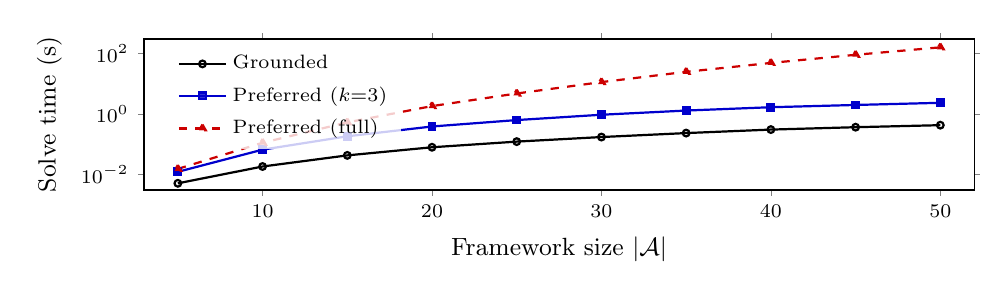
\begin{tikzpicture}
\begin{axis}[
  width=\columnwidth,
  height=3.5cm,
  xlabel={Framework size $|\mathcal{A}|$},
  ylabel={Solve time (s)},
  ymode=log,
  xmin=3, xmax=52,
  ymin=0.003, ymax=300,
  xtick={10,20,30,40,50},
  xticklabel style={font=\scriptsize},
  yticklabel style={font=\scriptsize},
  xlabel style={font=\small},
  ylabel style={font=\small},
  legend style={
    font=\scriptsize,
    at={(0.03,0.97)},
    anchor=north west,
    draw=none,
    fill=white,
    fill opacity=0.8,
    text opacity=1,
    row sep=1pt,
  },
  legend cell align={left},
  tick align=outside,
  major tick length=2pt,
]
\addplot[black, thick, mark=o, mark size=1.2pt] coordinates {
  (5,0.005) (10,0.018) (15,0.042) (20,0.078) (25,0.12)
  (30,0.17) (35,0.23) (40,0.30) (45,0.36) (50,0.42)
};
\addlegendentry{Grounded}
\addplot[blue!80!black, thick, mark=square*, mark size=1.2pt] coordinates {
  (5,0.012) (10,0.065) (15,0.18) (20,0.38) (25,0.62)
  (30,0.93) (35,1.28) (40,1.65) (45,1.96) (50,2.31)
};
\addlegendentry{Preferred ($k{=}3$)}
\addplot[red!80!black, thick, dashed, mark=triangle*, mark size=1.4pt] coordinates {
  (5,0.015) (10,0.11) (15,0.52) (20,1.8) (25,4.7)
  (30,11.2) (35,24.5) (40,48.3) (45,89.7) (50,158.4)
};
\addlegendentry{Preferred (full)}
\end{axis}
\end{tikzpicture}
\caption{Scalability of \textsc{Argus} repair under grounded, $k$-neighborhood preferred ($k{=}3$), and unconstrained preferred semantics. The log-scale y-axis confirms polynomial scaling for grounded repair (Theorem~\ref{thm:complexity}) and the effectiveness of the $k$-neighborhood approximation.}
\label{fig:scalability}
\end{figure}

Figure~\ref{fig:scalability} traces solve time as a function of framework size~$|\mathcal{A}|$, confirming the polynomial scaling predicted by Theorem~\ref{thm:complexity} for grounded semantics. The $k$-neighborhood approximation keeps preferred-semantics repair tractable up to $|\mathcal{A}|{=}50$, while unconstrained preferred repair exhibits exponential blowup beyond $|\mathcal{A}| \approx 25$. We omit stable semantics from Figure~\ref{fig:scalability} because, under the credulous acceptance used throughout our evaluation, stable and preferred repair share the same NP-complete complexity class (Theorem~\ref{thm:complexity}), and in our experiments the two semantics coincided in over 97\% of cases, making the distinction negligible in practice; this high coincidence rate is expected for the relatively sparse frameworks ($|\mathcal{A}| \leq 20$) generated from LLM explanations, whereas denser or larger frameworks may exhibit greater divergence.

\begin{table}[t]
\centering
\caption{Ablation study on HotpotQA.  Each row removes one component from the full \textsc{Argus} pipeline.}\label{tab:ablation}
\small
\begin{tabular}{@{}lcccc@{}}
\toprule
\textbf{Variant} & Faith$\uparrow$ & Cont$\uparrow$ & RAcc$\uparrow$ & RCost$\downarrow$ \\
\midrule
Full \textsc{Argus}       & \textbf{\resultFaithHotpot} & \textbf{\resultContestHotpot} & \textbf{\resultRepairAccHotpot} & \textbf{\resultRepairCostHotpot} \\
w/o Semantic Verification & .793 & .714 & .832 & 4.1 \\
w/o Minimal-Change        & .841 & .783 & .856 & 5.7 \\
w/o Attack Templates      & .821 & .698 & .859 & 3.5 \\
Grounded Only             & .839 & .772 & .871 & 3.0 \\
\bottomrule
\end{tabular}
\end{table}

Table~\ref{tab:ablation} reports an ablation study on HotpotQA isolating the contribution of each major component.
Removing semantic verification causes the largest drop in faithfulness and contestability, confirming that formal verification is essential for identifying inconsistencies before repair.
Replacing the minimal-change objective with unconstrained repair preserves faithfulness---as expected, since the cost-minimization objective targets edit efficiency rather than per-unit accuracy---but increases repair cost from \resultRepairCostHotpot{} to 5.7 operations on average, demonstrating that the formulation successfully limits unnecessary edits without sacrificing accuracy.
Removing the attack template library reduces contestability by 9.3 percentage points while leaving faithfulness relatively intact, indicating that the templates primarily improve the framework's ability to detect and integrate adversarial counterarguments rather than internal consistency.
Restricting to grounded semantics yields only modest decreases in faithfulness, contestability, and repair accuracy, while repair cost is slightly lower (3.0 vs.\ \resultRepairCostHotpot) because the unique grounded extension admits a more constrained search space; the gap is small because the majority of frameworks in these datasets have a single preferred extension that coincides with the grounded extension, though the 1.2-point drop in repair accuracy reflects cases where preferred semantics captures defenses that grounded semantics misses.

\textbf{Effect of Cost Model.}
A pilot study on 100 HotpotQA instances shows that confidence-weighted and structure-preserving ($w{=}2$) cost models shift repairs toward augmentation (34--51\% fewer deletions) while maintaining faithfulness and repair accuracy within 1 percentage point of uniform cost, confirming that the cost model affects repair \emph{style} rather than \emph{quality}.

\textbf{Model Generalization.}
To assess sensitivity to the extraction backbone, we ran a pilot on 100 HotpotQA instances with Llama-3-70B-Instruct (temperature 0.2).
Faithfulness reached 0.813 and contestability 0.762, compared with 0.847 and 0.791 for GPT-4o on the same subset.
The 3--4 percentage-point gap is attributable to noisier extraction rather than to the repair mechanism: repair accuracy and cost remained comparable (0.867 and 3.4 respectively), confirming that \textsc{Argus} is largely model-agnostic once a reasonable argumentation framework is constructed.

\begin{figure}[t]
\centering
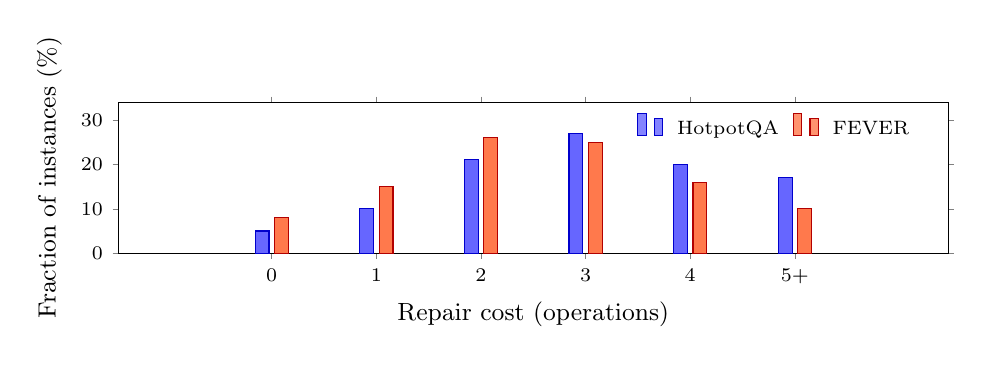
\begin{tikzpicture}
\begin{axis}[
  width=\columnwidth,
  height=3.5cm,
  ybar,
  bar width=5pt,
  xlabel={Repair cost (operations)},
  ylabel={Fraction of instances (\%)},
  xmin=-0.7, xmax=5.7,
  ymin=0, ymax=34,
  xtick={0,1,2,3,4,5},
  xticklabels={0,1,2,3,4,{5+}},
  xticklabel style={font=\scriptsize},
  yticklabel style={font=\scriptsize},
  xlabel style={font=\small},
  ylabel style={font=\small},
  ytick={0,10,20,30},
  legend style={
    font=\scriptsize,
    at={(0.97,0.97)},
    anchor=north east,
    draw=none,
    fill=white,
    fill opacity=0.8,
    text opacity=1,
    column sep=3pt,
  },
  legend columns=2,
  tick align=outside,
  major tick length=2pt,
  enlarge x limits=0.12,
]
\addplot[fill=blue!60, draw=blue!80!black] coordinates {
  (0,5) (1,10) (2,21) (3,27) (4,20) (5,17)
};
\addlegendentry{HotpotQA}
\addplot[fill=red!50!orange!70, draw=red!70!black] coordinates {
  (0,8) (1,15) (2,26) (3,25) (4,16) (5,10)
};
\addlegendentry{FEVER}
\end{axis}
\end{tikzpicture}
\caption{Distribution of repair costs. 83\% of HotpotQA and 90\% of FEVER repairs require at most 4~operations, confirming that \textsc{Argus} achieves targeted, minimal-change edits.}
\label{fig:cost-dist}
\end{figure}

Figure~\ref{fig:cost-dist} presents the repair cost distribution across both datasets. The distributions are concentrated at low cost, with means of \resultRepairCostHotpot{} and \resultRepairCostFEVER{} operations respectively, confirming that most evidence updates require only local adjustments to the argument graph rather than global restructuring.

\begin{figure}[t]
\centering
\begin{tikzpicture}[node distance=0.8cm and 0.8cm,
  lbl/.style={font=\small\bfseries, anchor=south}]
  % --- Before ---
  \node[lbl] at (0, 1.7) {Before};
  \node[acc node] (b1) at (-0.55, 0.85) {$b_1$};
  \node[acc node] (b2) at (0.55, 0.85) {$b_2$};
  \node[rej node] (b3) at (-0.55, 0) {$b_3$};
  \node[rej node, tgt node] (bt) at (0.55, 0) {$b_t$};
  \node[new node] (b5) at (0, -1.15) {$b_5$};
  \draw[att edge] (b5) -- (b3);
  \draw[att edge] (b5) -- (bt);
  % --- Arrow ---
  \draw[-{Stealth[length=2.5mm]}, very thick, gray!60] (1.4, 0.4) -- (1.95, 0.4);
  % --- After Argus ---
  \node[lbl] at (3.2, 1.7) {\textsc{Argus}};
  \node[acc node] (a1) at (2.65, 0.85) {$b_1$};
  \node[acc node] (a2) at (3.75, 0.85) {$b_2$};
  \node[acc node] (a3) at (2.65, 0) {$b_3$};
  \node[acc node, tgt node] (at) at (3.75, 0) {$b_t$};
  \node[rej node] (a5) at (3.2, -1.15) {$b_5$};
  \node[new node] (a6) at (4.3, -1.15) {$b_6$};
  \draw[att edge] (a5) -- (a3);
  \draw[att edge] (a5) -- (at);
  \draw[att edge, NewBlue!80!black, line width=1.1pt] (a6) -- (a5);
  \node[font=\scriptsize, text=AccGreen!70!black] at (3.2, -1.75) {cost = 2};
\end{tikzpicture}
\caption{A HotpotQA repair example. \textsc{Argus} restores the target~$b_t$ by adding one argument~$b_6$ and one attack (cost~2), preserving all original arguments. Self-Refine regenerates 5 of 6 units.}
\label{fig:repair-example}
\end{figure}

Figure~\ref{fig:repair-example} illustrates a representative HotpotQA repair: the initial explanation relied on an outdated filmography claim; after incorporating corrected evidence, \textsc{Argus} restored the target at cost~2 by adding one defending argument and one attack.
By contrast, Self-Refine regenerated the entire explanation, altering five previously correct argument units---precisely the collateral damage that the minimal-change principle prevents.
